\section{Experimentation and evaluation}

\subsection{First Experiment: With internet connection}
For this experiment both cloud servers were up and running and it were perfomed
99 iterations of requests. In each iteration was requested for every single one
of the serverless functions in \textit{sample\_functions} (see
\ref{overview:sample_functions} and \ref{impl:sample_functions}) to be executed.
The system has no knowledge of the environment. The aim here is to identify
that it is accomplishing the mentioned use cases \ref{usecases:forward_cloud},
\ref{usecases:forward_local}, and \ref{usecases:manual_forward}


It is expected that the proxy will forward requests for \textit{func\_light} to be
executed locally, for \textit{func\_heavy} requests to be executed either locally
or in the cloud. It will depend on the impact of the connection latency, but
generally, the connection latency should be less than 1 second (difference in time
that takes for the function to execute locally and remotely), which means that the expected result is for the proxy to choose to forward to one of the cloud servers.
\textit{func\_super\_heavy} is expected to be executed in the cloud most of the
times, due to the big difference in time taken, and the function
\textit{func\_obese\_heavy} should always be executed in the London server because
it is configured that way. Apart from \textit{func\_obese\_heavy}, some
exploration is expected for each of the different environments and not only
exploitation of the runtime environment that the system considers as the best
option. Because of the latency verified in \ref{res:conn_latency}, when choosing
between one of the servers, it should choose the Frankfurt server, because it is
the one with less latency (despite being physically further).

\subsubsection{Results}

%\begin{table}[]
%\centering
%\caption{Results of 1st experiment.}
%\label{tab:first_exp_results}
%\footnotesize
%\begin{tabular}{cl|c|c|c|c|}
%\cline{3-6}
%\multicolumn{1}{l}{}                                               &               & \multicolumn{1}{l|}{\textbf{func\_light}} & \multicolumn{1}{l|}{\textbf{func\_heavy}} & \multicolumn{1}{l|}{\textbf{func\_super\_heavy}} & \multicolumn{1}{l|}{\textbf{func\_obese\_heavy}} \\ \hline
%\multicolumn{1}{|c|}{\multirow{2}{*}{\textbf{local}}}              & avg. time (s) & 0.085602                                  & 2.111840                                  & 4.100240                                         & -                                                \\ \cline{2-6} 
%\multicolumn{1}{|c|}{}                                             & count         & 94                                        & 20                                        & 25                                               & -                                                \\ \hline
%\multicolumn{1}{|c|}{\multirow{2}{*}{\textbf{London's server}}}    & avg. time (s) & 3.423012                                  & 5.741277                                  & 6.169448                                         & 3.384546                                         \\ \cline{2-6} 
%\multicolumn{1}{|c|}{}                                             & count         & 3                                         & 10                                        & 20                                               & 99                                               \\ \hline
%\multicolumn{1}{|c|}{\multirow{2}{*}{\textbf{Frankfurt's server}}} & avg. time (s) & 0.336398                                  & 1.253591                                  & 2.265615                                         & -                                                \\ \cline{2-6} 
%\multicolumn{1}{|c|}{}                                             & count         & 2                                         & 69                                        & 54                                               & -                                                \\ \hline
%\end{tabular}
%\end{table}

The obtained results, see Table \ref{tab:first_exp_results}, match the expected
results. For \textit{func\_light}, the time taken was so small (less than 1/10 of
a second) that proxy imediatly converged in the best option. The results for the
execution of the function \textit{func\_light} translate the results expected for
use case \ref{usecases:forward_local}.

For \textit{func\_heavy} and \textit{func\_super\_heavy}, it kept a ratio of
exploration vs exploitation of 3/7 and 5/6, respectively, but always choosing the
fastest of the cloud servers. The exploration rate also increases with the
duration of the execution, meaning that the proxy will look for better options the
longer it takes for a function to execute. The results for these two functions
correspond to the ones expected in use case \ref{usecases:forward_cloud}.

Also, as expected, \textit{func\_obese\_heavy} had a 100\% accuracy, thus matching
the expected outcome stated in use case \ref{usecases:manual_forward}.

\subsection{Second Experiment: Without internet connection to the servers}
For this experiment, both servers were turned off and the internet connection was
cut, leaving the system only operational locally. The system still keeps all the
knowledge acquired in the previous experiment.
The aim here is to identify that it is accomplishing the use case
\ref{usecases:fallback}.

In this experiment, it is expected for the weighting algorithm to suggest
executing the serverless function in one of the cloud servers, because it will
lead to a faster execution. Because there is no internet connection, it is
expected for the proxy to try to execute the function remotely, fail, and then to
fall back to the local runtime environment. In the end, the function should be
executed in the local runtime environment leading to the request being answered
successfully.

\subsubsection{Results}
First, the function \textit{weight\_scale} is queried to know which of the runtime
environments the proxy is going to choose (because the proxy chooses the runtime environment with less weight, knowing the weights allow us to know which option
the proxy is going to take). Because there is more information about the system,
the weighting algorithm used was the Bayesian UCB. As it can be seen in the Listing
\ref{listing:exp_weight_query}, the runtime environment that is going to be
chosen is the Frankfurt's server.

\begin{listing}
\begin{lstlisting}[language=json, basicstyle=\footnotesize]
{
    "status": "success",
    "londonServer": 3.5747403999957266,
    "frankfurtServer": 1.1756422708191938,
    "local": 2.090245031544607
}

\end{lstlisting}
\caption{}
\label{listing:exp_weight_query}
\end{listing}

Even though the chosen runtime environment was Frankfurt's server, because there
was no internet connection it had to fall back to execute the function locally in
order to complete the request successfully, as seen in Listing
\ref{listing:exp_fallback_result}. The observed results match the ones expected
and also the proxy proceeded as stated in use case \ref{usecases:fallback}.

\begin{listing}
\begin{lstlisting}[language=json, basicstyle=\footnotesize]
{
    "nodeInfo": "61e20a65b48e ",
    "swarm": "local",
    "message": "I was able to achieve this result 
    using HEAVY calculations",
    "status": "The light is ON"
}
\end{lstlisting}
\caption{The request was executed locally, as indicated by the key \textit{swarm},
which is the swarm (runtime environment) where the function was executed.
\textit{local}, is the name given to the local network of devices, as configured
when setting up the proxy.}
\label{listing:exp_fallback_result}
\end{listing}


\subsection{Third Experiment: Turning off Internet connection in a series of requests}
During this experiment, the main purpose is to run a cycle of requests and then
turn off the Internet access in the middle of the cycle to observe how this will
affect response times. It will be run 99 iterations of requests and in each
iteration, it will be requested the execution of \textit{func\_heavy}, After
request number \textit{50}, the Internet connection will be cut off, leaving the
system only operational locally. The system will keep all the knowledge gathered
in the previous experiments. The aim here is to identify that it is accomplishing
the use case \ref{usecases:fallback} and how results vary throughout.

In this experiment, it is expected for the weighting algorithm to suggest
executing the serverless function in one of the cloud servers, because it will
lead to a faster execution. Because of this, the mean total time of the request should
be smaller in the first 50 requests. After the 50th request, because the internet
connection was cut off, the proxy will try to execute the function remotely, fail,
then fallback to execute the function locally, resulting in a larger mean total
time. 

\subsubsection{Results}

\begin{figure}[h]
  \begin{center}
    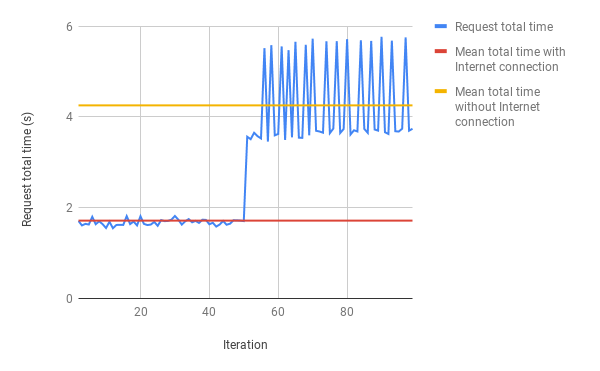
\includegraphics[width=0.5\textwidth]{exp3_chart.png}
    \caption{Chart illustrating the results of the third experience.}
    \label{fig:exp3_chart}
  \end{center}
\end{figure}

The obtained results, illustrated in Figure \ref{fig:exp3_chart}, match the
expected results. The mean total time of the request when there was Internet
connection was \textbf{1,71466602} seconds, and, at iteration number 50, it
jumped to \textbf{4,253785939} seconds when the Internet connection was cut off.
Despite having no internet connection, the system was still able to complete the
request, just with an added delay. The added delay was due to the fact that it had
to try to execute the function remotely and also because of the increased time it
takes to execute the function locally (2 seconds). The complete list of results
gathered from this experiment can be found in \ref{ap1:3rd_exp_complete_results}.

\subsection{Fourth Experiment: Adapting to lag}
\label{res:exp4}
In this experiment, it is going to be executed a series of requests and after
reaching to a while, the Internet connection is going to be purposely slowed to
see how the system reacts in situations of lag and slow connection. It will be run
249 iterations of requests and in each iteration it will be requested the
execution of \textit{func\_heavy}, After request number \textit{50}, the Internet
connection will be slowed down (\textbf{28 kbps UP, 14 kbps DOWN}) and the system
will continue to be asked to execute the functions. The system will have none of
the knowledge gathered in the previous experiments. The aim here is to identify
that it is accomplishing the use cases \ref{usecases:forward_cloud} and
\ref{usecases:forward_local}, and also that it is capable of adapting to changes
in the network.

In this experiment, it is expected that the system goes through three phases. In
the first phase, in the first 50 iterations, while the connection to the server is
working as expected, the system is supposed to gather information about the
environment and to converge to the best option (one of the cloud servers).

In the second phase, the Internet connection is slowed down and the execution of
function remotely should take longer than the execution of the function locally.
In this phase, the system is supposed to still converge to one of the cloud
servers but gradually diminishing the frequency in which it chooses the cloud
serves as the best option.

After this phase, the system will enter the third phase where the results gathered
after the introduction of network lag outweigh the results gathered in the first
phase. Here, the system should start to converge to the local network as the
best option.


\subsubsection{Final Remarks}

\begin{figure}[h]
  \begin{center}
    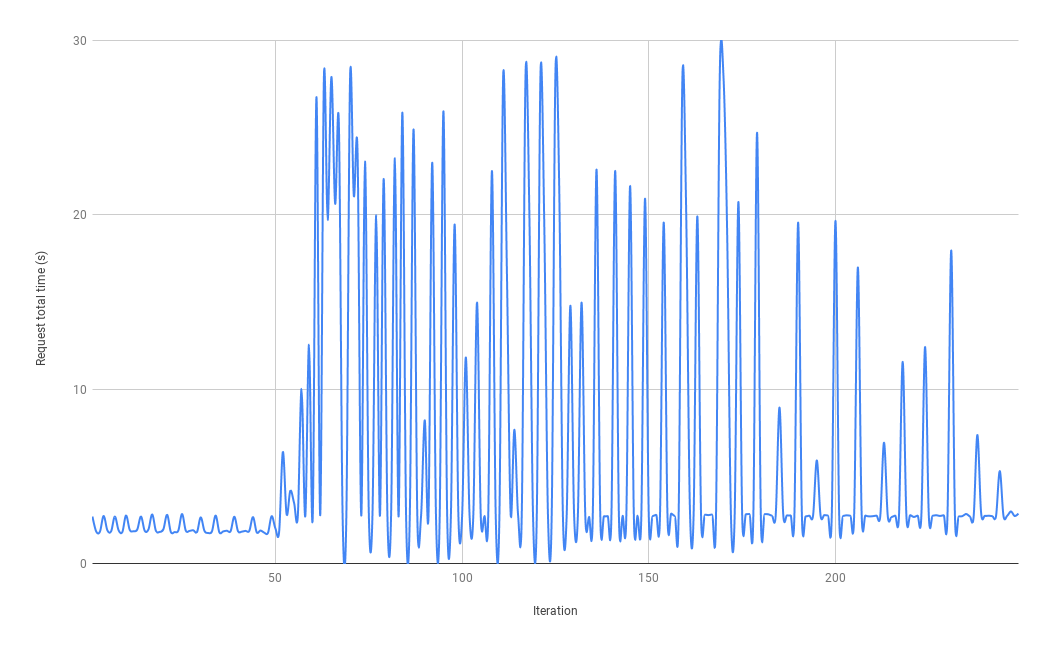
\includegraphics[width=0.5\textwidth]{exp4_total_time_chart.png}
    \caption{Requests total time throughout the various iterations of the
    fourth experiment.}
    \label{fig:exp4_total_time_chart}
  \end{center}
\end{figure}


The gathered results can be observed in Figure \ref{fig:exp4_total_time_chart}. As
expected, the results for the first 50 iterations are the expected results in a
standard situation. After the introduction of network lag, we start to observe
spikes in the total time it takes for the function to be executed. These spikes
refer to the execution of the function remotely. In the first 30/40 requests after
the introduction of network lag (iterations 50 to 90), the frequency of requests
that are executed remotely is still high. The frequency starts to diminish
from that point on and at around iteration 175 the system starts to choose the
local network more frequently than the cloud servers.

\begin{figure}[h]
  \begin{center}
    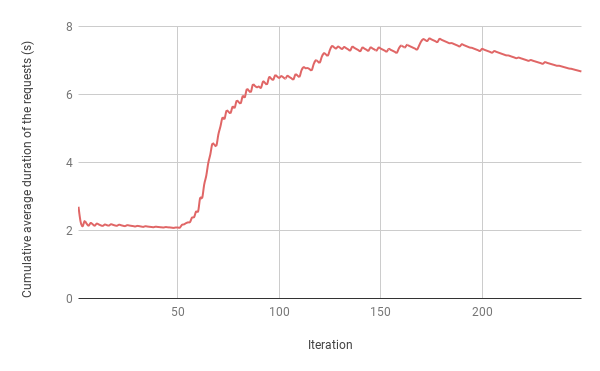
\includegraphics[width=0.5\textwidth]{exp4_avg_chart.png}
    \caption{Cumulative average duration of the request throughout the various iterations of the fourth experiment. E.g., the value in iteration 50 (2.085604 seconds) is the average duration of the first 50 requests.}
    \label{fig:exp4_avg_chart}
  \end{center}
\end{figure}

Figure \ref{fig:exp4_avg_chart}, shows a different perspective of the results,
showing the cumulative average duration of the requests throughout the experiment.
It can be seen here that around iteration 175 the system changed course and
started to converge to the local network as the best option. This marks the point
where the system finally adapted to the changes introduced.

The various phases can be seen more easily here, in Figure
\ref{fig:exp4_avg_chart}. The first phase can be seen from iteration 0 to 50, the
second phase from iteration 50 to 175, and the third phase from iteration 175 to
250.

Nevertheless, it took around 125 iterations (from iteration 50 to iteration 175)
for the system to adapt. After 50 iterations where the system gathered information
that became invalid, it took the system 250\% more iterations to adapt to the new
conditions. These results show that the system, although capable of adapting, will
take a considerable amount of time to adapt to new conditions.
